\documentclass[11pt]{article}
\usepackage[T1]{fontenc}
\usepackage{amsmath,amssymb,amsthm,mathtools}
\usepackage[margin=1.1in]{geometry}
\usepackage{natbib}
\usepackage{booktabs,longtable,array,tabularx}
\usepackage{tikz}
\usetikzlibrary{positioning,arrows.meta,calc}
\usepackage{placeins}
\tikzset{
  audit/node/.style={rectangle,draw=black,rounded corners=1.5pt,
    text width=3.65cm,minimum height=0.95cm,inner sep=4pt,
    align=center,font=\footnotesize,fill=white},
  audit/refuted/.style={audit/node,line width=0.8pt,fill=black!7},
  audit/qualified/.style={audit/node,dashed,fill=black!3},
  audit/edge/.style={-{Stealth[length=1.8mm,width=1.3mm]},
    draw=black,line width=0.45pt,rounded corners=2pt},
  audit/note/.style={font=\scriptsize,fill=white,inner sep=1.2pt,align=center}
}
\usepackage{hyperref}
\hypersetup{colorlinks=true,linkcolor=blue,citecolor=blue,urlcolor=blue}
\setlength{\emergencystretch}{1em}
\newtheorem{theorem}{Theorem}
\newtheorem{proposition}[theorem]{Proposition}
\newtheorem{lemma}[theorem]{Lemma}
\newtheorem{corollary}[theorem]{Corollary}
\theoremstyle{remark}\newtheorem{remark}[theorem]{Remark}
\newcommand{\R}{\mathbb R}
\newcommand{\ind}{\mathbf 1}
\newcommand{\G}{\mathcal G}
\newcommand{\X}{\mathcal X}
\newcommand{\norm}[1]{\lVert#1\rVert}
\title{Measurable Deviations:\\ A Comment on ``The Converse Envelope Theorem''}
\author{Shuo Li Liu}
\date{25 October 2026}
\begin{document}
\maketitle
\begin{abstract}
An optimal rule may satisfy the envelope formula, while shifted versions of its payoffs lack Lebesgue integrability, even when the action space is compact and the payoff functions are jointly continuous. We establish the shifted-integral identity for measurable paths of differentiable payoff profiles with a common Lipschitz bound and continuous selected value. Further counterexamples reveal flaws in an auxiliary absolute continuity equivalence, an approximation lemma, the literal strict outer condition and a uniform convergence claim about information distributions. We delimit their consequences and establish a narrower continuity result for binary information. Counterexamples and repairs are proved using Lean~4.
\end{abstract}
\noindent\textit{Keywords:} envelope theorem, incentive compatibility, measurability, payoff profiles.\par
\noindent\textit{JEL classification:} C61, D82.

\section{The missing integral domain}
The converse envelope theorem of \citet{Sinander2022} characterizes the envelope formula through a derivative of integrated payoffs from shifted decision rules. Fixed-action type regularity does not ensure measurability of these payoffs. Our counterexample challenges the claimed well-definedness of this outer condition \citep[Section 1]{Sinander2022}, even with compact actions and continuous payoffs. Section~\ref{sec:repair} gives a sufficient measurable-profile repair; Section~\ref{sec:scope} identifies four separate defects and their limits. Proof dependencies and further details appear in the appendices.

\subsection{Formulation}
Let $T=[0,1]$, let $\X$ be a set, and let $f:\X\times T\to\R$. A decision rule $X:T\to\X$ induces
\[
 V(s)=f(X(s),s),\qquad D(s)=f_2(X(s),s),
\]
where $f_2$ denotes the interior type derivative; no endpoint derivative is required. For $0<r<t<1$ and shifts keeping $[r+h,t+h]\subset T$, set
\begin{equation}\label{eq:J}
 J_{r,t}(h)=\int_r^t f(X(s+h),s)\,ds.
\end{equation}
The outer first-order condition is $J_{r,t}'(0)=0$ for every interior interval; it requires $J_{r,t}$ to exist near zero. All substantive integral assertions concern integrable functions and ordinary Lebesgue integrals.

The integral envelope identity is
\begin{equation}\label{eq:env}
 V(t)-V(r)=\int_r^t D(s)\,ds.
\end{equation}
The basic assumptions in \citet[Sections 2--3]{Sinander2022} require fixed-action type derivatives and absolute equicontinuity. ``Outer'' concerns the order of differentiation and integration, not outer integration.

\subsection{The counterexample}
Choose a non-Lebesgue-measurable rational-equivalence transversal $A\subset[1/3,2/3]$. Fix $r=1/4$ and $t=3/4$.

\begin{theorem}[A smooth envelope with undefined shifted integrals]\label{thm:counter}
There are payoffs on the nominal action set $[0,1]^2$ and an everywhere optimal rule such that every fixed-action profile is differentiable and $2$-Lipschitz, $V=D=0$, and the integrand in \eqref{eq:J} is not Lebesgue measurable for every $0<|h|<1/12$.
\end{theorem}
\begin{proof}
For $x=(u,y)$ define
\[
 f((u,y),s)=-\ind_A(y)(s-u)^2,\qquad X(s)=(s,s).
\]
Each profile is polynomial, with derivative $-2\ind_A(y)(s-u)$ bounded in absolute value by $2$ on $T$. For $h\ne0$, the divided-difference supremum is
\[
 \sup_{(u,y)\in[0,1]^2}\left|\frac{f((u,y),s+h)-f((u,y),s)}h\right|
 =\max\{|2s+h|,|2s+h-2|\}.
\]
Since $A\ne\varnothing$, the coefficient can equal $1$; the remaining absolute affine expression is maximized at an endpoint in $u$. The displayed function is continuous and bounded by $2$ when $s,s+h\in T$. Zero extension outside this domain gives a measurable, uniformly integrable family, verifying absolute equicontinuity.

Nonpositive payoffs and $V=D=0$ give optimality and \eqref{eq:env}.

For a nonzero shift,
\[
 f(X(s+h),s)=-h^2\ind_A(s+h).
\]
For $0<|h|<1/12$, the set $A-h$ lies in $[r,t]$. Measurability there, division by $-h^2$, and extension by zero would make $\ind_{A-h}$ measurable on $\R$. Translation would make $A$ measurable, a contradiction.
\end{proof}

\begin{proposition}[Compact actions do not regularize every selector]\label{prop:compactexample}
The same failure is possible with a compact metric action space and a jointly continuous payoff, although a measurable optimal selector also exists.
\end{proposition}
\begin{proof}
Take $\X=[0,1]\times\{0,1\}$ and
\[
 F((u,c),s)=-c(s-u)^2,\qquad \widehat X(s)=(s,\ind_A(s)).
\]
The payoff is jointly continuous and the preceding calculations apply. The constant rule $s\mapsto(0,0)$ is also optimal and has zero deviation payoffs.
\end{proof}

\paragraph{Where domination stops.}
Let
\[
 \begin{aligned}
 \phi_h(s)&=\frac{V(s+h)-V(s)}h,\\
 \psi_h(s)&=\frac{f(X(s+h),s+h)-f(X(s+h),s)}h,\\
 \chi_h(s)&=\frac{f(X(s+h),s)-f(X(s),s)}h.
 \end{aligned}
\]
Here $\phi_h=\psi_h+\chi_h$, while the example gives $0=h\ind_A(s+h)-h\ind_A(s+h)$. The nonmeasurable components cancel. Domination alone therefore cannot justify their $L^1$ membership in the Identity Lemma (unnumbered, Appendix~A.3) or Lemma~2 (Appendix~A.4) of \citet{Sinander2022}.

\section{A sufficient repair}\label{sec:repair}
Put $C=C([0,1],\R)$ with the supremum norm and let
\[
 \Phi(x)=f(x,\cdot),\qquad g(s)=\Phi(X(s)).
\]
We require Borel measurability of $g$, without prescribing a topology on action labels. Appendix~\ref{app:representation} gives verification criteria and compactness results for selected profiles.

\begin{theorem}[The repaired identity]\label{thm:identity}
Let $g:T\to C$ be Borel measurable. Suppose every profile is $L$-Lipschitz and differentiable at each interior type. Suppose also that $V(s)=g(s)(s)$ is continuous. Put $D(s)=g(s)'(s)$ in the interior, with endpoint values zero. For $0<r<t<1$, the shifted integral \eqref{eq:J}, interpreted as $\int_r^t g(s+h)(s)\,ds$, is well-defined near zero and
\begin{equation}\label{eq:identity}
 J_{r,t}'(0)=V(t)-V(r)-\int_r^t D(s)\,ds.
\end{equation}
\end{theorem}
\begin{proof}
Proposition~\ref{prop:measeval} gives measurable composites. Boundedness of $V$ and $|g(s+h)(s)-V(s+h)|\le L|h|$ give integrability near zero shift. Measurable backward profile quotients at steps $1/n$, set to zero where the step leaves $T$, converge pointwise to $D$ in the interior. Thus $D$ is measurable and $|D|\le L$.

Change variables $u=s+h$ and set
\[
 q_h(u)=\frac{g(u)(u-h)-V(u)}h.
\]
For small nonzero $h$,
\[
 \frac{J_{r,t}(h)-J_{r,t}(0)}h
 =\frac{\int_{r+h}^{t+h}V(u)\,du-\int_r^tV(u)\,du}h
   +\int_{r+h}^{t+h}q_h(u)\,du.
\]
By continuity of $V$, the first term tends to $V(t)-V(r)$. On a compact interior interval containing all shifted intervals for sufficiently small shifts, $q_h$ is measurable, $|q_h|\le L$, and $q_h(u)\to-D(u)$. Hence $\ind_{[r+h,t+h]}q_h\to-\ind_{[r,t]}D$ almost everywhere. Dominated convergence gives the second term's limit and the two-sided derivative.
\end{proof}

\begin{corollary}[Converse on the repaired domain]\label{cor:converse}
Under Theorem~\ref{thm:identity}, the outer first-order condition on every interior interval is equivalent to the integral envelope identity on those intervals. The identity then extends to the endpoints and implies absolute continuity of $V$.
\end{corollary}
\begin{proof}
Equation~\eqref{eq:identity} gives the equivalence. Continuity of $V$ and $|D|\le L$ extend it to endpoints, representing $V$ as a constant plus an indefinite integral of an integrable function.
\end{proof}

\paragraph{Extent of the repair.}
The theorem derives integrability of $D$; the outer condition then gives absolute continuity of $V$. The repair uses a common Lipschitz bound and continuous $V$, so it does not cover full absolute equicontinuity. Profile measurability is sufficient; its necessity is not established. No necessity of Standard Borel actions or exclusion of nonseparable models follows.

\paragraph{What integrability alone repairs.}
Requiring $s\mapsto f(X(s+h),s)$ to be Lebesgue integrable on every interior interval for all sufficiently small admissible shifts makes $J_{r,t}$ well-defined near zero and excludes the rule in Theorem~\ref{thm:counter}. All four independent defects in Section~\ref{sec:scope} remain: the approximation obstruction is topological, while the spike, strict-condition, and Supplement~S.2 witnesses already have finite integrals. The spike refutes the auxiliary implication from uniform integrability to absolute continuity; the main equivalence excludes it through its absolute-continuity premise. Whether this amendment alone suffices for that equivalence under full absolute equicontinuity is not established here.

\paragraph{Induced structure and admissibility.}
The claim that the theorem ``requires no structure on the choice set'' \citep[Abstract]{Sinander2022} does not preclude structure induced by its payoff assumptions. Continuous fixed-action profiles induce a supremum metric on payoff-equivalence classes; uniform equicontinuity and bounded diagonal values give compact closure of the selected profiles (Appendix~\ref{app:representation}). This geometry does not ensure measurability of the selected profile path. Indeed, Proposition~\ref{prop:compactexample} gives compact metric actions and jointly continuous payoffs, yet an everywhere-optimal rule with $V=D=0$ has undefined shifted integrals. Requiring shifted-payoff integrability therefore excludes some optimal rules admitted by the basic assumptions. The demonstrated gap concerns the claimed unrestricted well-definedness of the outer condition \citep[Section~1]{Sinander2022}; no necessity of a prescribed topology on action labels follows.

\section{Scope of the corrections}\label{sec:scope}
Appendix~\ref{app:dependency} maps the affected proof steps; Appendix~\ref{app:audit-witnesses} proves the following four findings.

\paragraph{Absolute continuity of an arbitrary selected value.}
For $f(x,t)=x$ on $\{0,1\}$ and $X(t)=\ind_{\{1/2\}}(t)$, shifted integrals vanish and imitation quotients are uniformly integrable, but $V=X$ is discontinuous. The envelope equality at $1/2$, normalized at zero, has sides $1$ and $0$. This refutes Lemma~2(ii)$\Rightarrow$(i), the corresponding Lemma~4 implication, and Appendix~A.7's weakening. The main equivalence excludes this rule through its explicit absolute-continuity premise. Lemma~3 derives absolute continuity from optimality; A.7 is not used by the main or implementability theorem. The forward envelope conclusion of \citet{MilgromSegal2002} remains valid.

\paragraph{The topology used for approximation.}
Four strict order rays isolate each point of coordinatewise ordered $\R^2$, making the ambient and inherited chain topologies discrete. Thus $Y(t)=(t,0)$ has no continuous endpoint-preserving approximation from $[0,1]$. This refutes the approximation lemma and invalidates its use in Step~2 of the implementability proof. It does not refute the implementability conclusion. An intrinsic-chain-topology repair would need preference continuity in that topology too. We do not give that general repair here.

\paragraph{The literal strict outer condition.}
Constant allocation and payment paths are weakly increasing. With continuous fixed-outcome/payment type profiles, their shifted integrals exist and their outer derivatives vanish. They violate Definition~7's strict implication $q(n)\ge0\Rightarrow q(n')>0$ for $n<n'$. The universal strict condition is therefore impossible on nonempty outcome spaces under these assumptions, even when restricted to integrable paths. Neither the nonstrict condition nor classical strict single crossing is refuted.

\paragraph{Uniform convergence in the information application.}
With binary posterior space $[0,1]$ and prior $p=1/2$, let
\[
 y=\delta_p,\qquad y_n=\tfrac12\delta_{p-\varepsilon_n}
                 +\tfrac12\delta_{p+\varepsilon_n},
 \qquad \varepsilon_n=\frac1{4(n+1)}.
\]
These laws form a Blackwell chain converging to $y$ in the full ambient strict-ray topology and its inherited chain topology. Yet the supremum discrepancy over differences $w=v^+-v^-$ of continuous convex functions with $|w|\le1$ equals $2$ for every $n$. All integrals are finite. This refutes Supplement Lemma~S.2. Uniform convergence over normalized continuous \emph{convex} tests does hold. For payoffs continuous and convex in the posterior with a common type-Lipschitz bound, it yields joint continuity of expected payoffs and of their continuous monetary aggregations. Appendix~\ref{app:audit-dc-tests} proves this binary, prior-$1/2$ repair; it does not establish the general finite-state application or repair the approximation and strictness defects.

\appendix
\section{Payoff representation and compactness}\label{app:representation}\subsection{Measurability criteria}
Put $C=C(T,\R)$ with its supremum norm. Whenever fixed-action profiles are continuous, define
\[
 \Phi(x)=f(x,\cdot),\qquad g(s)=\Phi(X(s)),\qquad
 \G=\{g(s):s\in T\}.
\]
Equality under $\Phi$ defines payoff equivalence; the map identifies the resulting quotient with its image. No topology on action labels is assumed.

\begin{proposition}[Measurable evaluation]\label{prop:measeval}
Let $(S,\Sigma)$ be any measurable space. If $p:S\to C$ and $\tau:S\to T$ are measurable for the respective Borel structures, then $s\mapsto p(s)(\tau(s))$ is measurable. Consequently, if $g:T\to C$ is Borel measurable and $\sigma,\tau:S\to T$ are measurable into the Borel sigma algebra of $T$, then $s\mapsto g(\sigma(s))(\tau(s))$ is measurable. If its absolute value is bounded on a measurable set of finite measure, it is integrable there.
\end{proposition}
\begin{proof}
Evaluation $C\times T\to\R$, $(p,t)\mapsto p(t)$, is continuous by the triangle inequality, supremum-norm convergence, and continuity of the limiting profile. Since $C([0,1])$ and $[0,1]$ are separable metric spaces, their product Borel sigma algebra equals the product sigma algebra. Compose evaluation with the measurable pair $(p,\tau)$ or $(g\circ\sigma,\tau)$, then apply bounded integrability on a finite-measure set.
\end{proof}

\begin{theorem}[Countable tests on a compact family]\label{thm:tests}
Let $K\subset C$ be compact and let $(q_n)_{n\ge1}$ have dense range in $T$. For any measurable space $S$ and map $g:S\to K$,
\[
 g\text{ is Borel measurable}\quad\Longleftrightarrow\quad
 s\mapsto g(s)(q_n)\text{ is measurable for every }n.
\]
\end{theorem}
\begin{proof}
The evaluation map $e:K\to\R^{\mathbb N}$, $e(p)=(p(q_n))_n$, is continuous for the product topology and injective by density. Compactness and Hausdorffness make it a homeomorphism onto its closed image, with measurable inverse. Thus $e\circ g$ is measurable exactly when its coordinates are measurable, proving the equivalence.
\end{proof}

\begin{proposition}[An action-space alternative]\label{prop:caratheodory}
Suppose $\X$ carries any sigma algebra, $f(x,\cdot)$ is continuous, and $f(\cdot,t)$ is measurable for each $t$. If a chosen rule $X$ is measurable, its payoff evaluated along any measurable type path is measurable. No Standard Borel or separability assumption on $\X$ is required.
\end{proposition}
\begin{proof}
For Carath\'eodory measurability, approximate the identity on the separable metric type interval by countably valued measurable maps. Continuity in type gives joint measurability by pointwise convergence; compose with the selected action and type paths.
\end{proof}

\subsection{Compact profiles from bounded diagonal payoffs}
Compactness alone does not make the selected profile path measurable.

\begin{theorem}[Anchored compactness]\label{thm:ascoli}
Suppose the family $\{g(s):s\in T\}$ is uniformly equicontinuous and
\[
 |g(s)(s)|\le M\quad(s\in T)
\]
for some finite $M$. Then this family is uniformly bounded, and $K=\overline\G$ is compact in $C$. In particular, a continuous diagonal value suffices for the bound.
\end{theorem}
\begin{proof}
Choose $\delta>0$ such that $|p(u)-p(v)|<1$ for every $p\in\G$ whenever $|u-v|<\delta$, and an integer $N$ with $1/N<\delta$. Join any two points of $T$ by $N$ equal increments shorter than $\delta$ to obtain $|p(u)-p(v)|\le N$. For $p=g(s)$, the anchor bound $|p(s)|\le M$ gives $|p(u)|\le M+N$ for every $u$. Arzel\`a--Ascoli gives compact closure. A continuous diagonal is bounded on compact $T$.
\end{proof}

On a disconnected compact domain, equicontinuity and a bounded moving anchor need not give a uniform bound. Under a shared $L$-Lipschitz bound on $T$, $\norm{g(s)}_\infty\le M+L$.

\begin{corollary}[Compact convexification]\label{cor:convex}
Under Theorem~\ref{thm:ascoli}, the closed convex hull of $\G$ in $C$ is compact and convex.
\end{corollary}
\begin{proof}
Convex combinations of a finite $\varepsilon$-net for $\G$ approximate those from $\G$ within $\varepsilon$. The finite net's convex hull is compact and has a finite $\varepsilon$-net, so the convex hull of $\G$ is totally bounded. Completeness of $C$ makes its closure compact; convexity is preserved under closure.
\end{proof}

To read the corollary as a statement about lotteries, those lotteries must be feasible and their payoff profiles must equal the corresponding averages. The corollary neither imposes convexity on the action set nor recovers classical differentiability of a decision rule. Theorem~\ref{thm:ascoli} does not establish measurability of $g$, as Proposition~\ref{prop:compactexample} shows within a compact profile family. Although the compact closure $K$ is standard Borel, an arbitrary subset $\G$ need not be Borel in it.

Continuous payoff profiles thus induce metric geometry on payoff-equivalence classes. Under uniform equicontinuity, bounded implemented values yield compact closure of the selected profile family. These consequences of the payoff assumptions also hold in forward-envelope environments under those assumptions; they do not require a prescribed topology on action labels. We can use this representation to state and check path measurability. The counterexample shows why the unrestricted ordinary-integral formulation needs an admissibility restriction. The induced topology alone does not show that.


\FloatBarrier
\section{Proof dependencies and assessed scope}\label{app:dependency}
The maps and tables follow the numbering of the article \citep{Sinander2022} and online supplement \citep{Sinander2022supp}. An arrow says where a published proof uses another result. A lemma that fails in general may still apply under stronger hypotheses. Tables expand the diagrams' abbreviated hypotheses. Appendix~\ref{app:audit-witnesses} proves additional counterexamples and specifies their scope; Appendix~\ref{app:formal} reports Lean certificates for the four counterexamples. We do not claim a formalization of every mapped source-paper result.


\subsection{Overview of affected claims}\label{app:audit-overview}
Figure~\ref{fig:audit-main} summarizes selected proof paths;
Table~\ref{tab:audit-impact} gives each objection's target and established
impact. Full maps and node-by-node tables follow.

\begin{figure}[htbp]
\centering
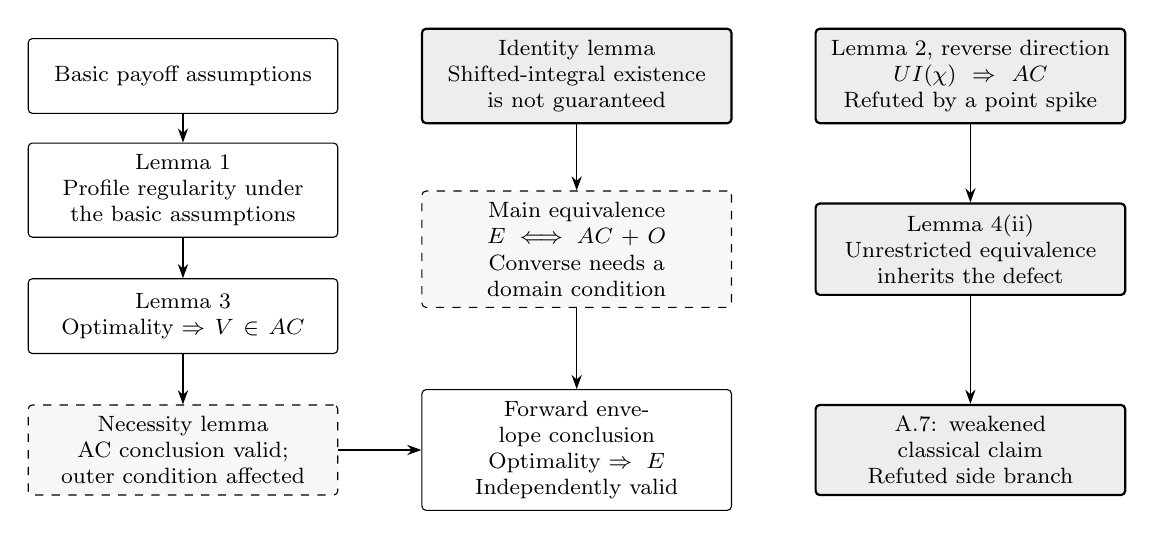
\begin{tikzpicture}
\node[audit/node] (mB) at (-5,0) {Basic payoff assumptions};
\node[audit/node] (mL1) at (-5,-1.45) {Lemma 1\\Profile regularity under the basic assumptions};
\node[audit/node] (mL3) at (-5,-3.05) {Lemma 3\\Optimality \(\Rightarrow V\in AC\)};
\node[audit/qualified] (mNec) at (-5,-4.75) {Necessity lemma\\AC conclusion valid;\\outer condition affected};
\node[audit/refuted] (mId) at (0,0) {Identity lemma\\Shifted-integral existence\\is not guaranteed};
\node[audit/qualified] (mMain) at (0,-2.2) {Main equivalence\\\(E\Longleftrightarrow AC+O\)\\Converse needs a domain condition};
\node[audit/node] (mForward) at (0,-4.75) {Forward envelope conclusion\\Optimality \(\Rightarrow E\)\\Independently valid};
\node[audit/refuted] (mL2) at (5,0) {Lemma 2, reverse direction\\\(UI(\chi)\Rightarrow AC\)\\Refuted by a point spike};
\node[audit/refuted] (mL4) at (5,-2.2) {Lemma 4(ii)\\Unrestricted equivalence\\inherits the defect};
\node[audit/refuted] (mWeak) at (5,-4.75) {A.7: weakened classical claim\\Refuted side branch};
\draw[audit/edge] (mB) -- (mL1);
\draw[audit/edge] (mL1) -- (mL3);
\draw[audit/edge] (mL3) -- (mNec);
\draw[audit/edge] (mId) -- (mMain);
\draw[audit/edge] (mMain) -- (mForward);
\draw[audit/edge] (mNec) -- (mForward);
\draw[audit/edge] (mL2) -- (mL4);
\draw[audit/edge] (mL4) -- (mWeak);
\end{tikzpicture}
\caption{Selected proof paths and counterexample scope.
\(E\) is the envelope formula, \(O\) the outer first-order condition,
and \(UI(\chi)\) uniform integrability of shifted payoff quotients.
Arrows record published dependencies, not propagation of falsity.
Lemma 3 gives absolute continuity from optimality; the main theorem does
not require Lemma 2's reverse direction. The A.7 weakening is a terminal
side claim. Lemma 4(i), the housekeeping lemma, the unaffected classical
special case, and further inputs appear in Figure~\ref{fig:audit-core}.}
\label{fig:audit-main}
\end{figure}

\begin{table}[htbp]
\centering
\small
\caption{Affected claims and the limits of each counterexample}
\label{tab:audit-impact}
\renewcommand{\arraystretch}{1.16}
\begin{tabularx}{\linewidth}{@{}>{\raggedright\arraybackslash}p{0.20\linewidth}>{\raggedright\arraybackslash}X>{\raggedright\arraybackslash}X@{}}
\toprule
Issue & Direct target in the original paper & Established impact \\
\midrule
Measurability of deviations & Lemma~2(i)$\Rightarrow$(ii), Identity Lemma, Necessity Lemma, main converse & An optimal rule satisfies the envelope formula with undefined shifted Lebesgue integrals. Theorem~\ref{thm:identity} restores the identity for measurable profiles with a common Lipschitz bound and continuous selected value. \\
Pointwise continuity & Lemma~2(ii)$\Rightarrow$(i), Lemma~4(ii), Appendix~A.7's weakening & All deviation integrals exist, but the envelope formula requires $1=0$. The main theorem's AC premise excludes the example. \\
Topology of chains & Approximation Lemma, proved in Supplement~S.3 & The continuous approximation need not exist, invalidating the general implementability proof's approximation step without refuting its conclusion. \\
Uniformity over convex differences & Supplementary Lemma~S.2 & The asserted vanishing supremum equals $2$. Preference continuity is proved independently for binary states with prior $1/2$ and a common type-Lipschitz bound. \\
Strict outer single crossing & Definition~7 and footnote~17 & Constant allocation and payment paths violate the literal strict condition; strict applications require a revised, nonvacuous premise. \\
\bottomrule
\end{tabularx}
\end{table}
\FloatBarrier

\subsection{Core theory}
\label{sec:audit-core-tables}

\paragraph{Notation.}
Types lie in $[0,1]$; integrals are ordinary Lebesgue integrals. Write
\[
 \begin{aligned}
 V(t)&=f(X(t),t),& D(t)&=f_2(X(t),t),\\
 \chi_h(s)&=\frac{f(X(s+h),s)-V(s)}{h},&
 J_{r,t}(h)&=\int_r^t f(X(s+h),s)\,ds.
 \end{aligned}
\]
$B$ denotes the basic assumptions: differentiability of each $f(x,\cdot)$
and uniform integrability of the actual family
$\Phi_h(s)=\sup_x|(f(x,s+h)-f(x,s))/h|$.
$C$ denotes the classical assumptions: a convex finite-dimensional action
set, an existing bounded action derivative, and a Lipschitz rule $X$.
$E$ is the pointwise integral envelope formula (Definition~2);
$O$ is $J'_{r,t}(0)=0$ on every interior interval (Definition~4);
$F$ requires the imitation derivative to exist and vanish almost everywhere
(Definition~3). AC means absolute continuity. UI requires $L^1$ membership,
hence measurability, and uniform absolute continuity of the integrals
(Definition~9).  The \emph{quadratic example} has $V=D=0$ but
nonmeasurable shifted payoffs; the \emph{spike example} is
$f(x,t)=x$, $X(t)=\mathbf 1_{\{1/2\}}(t)$.

\begin{figure}[p]
\centering
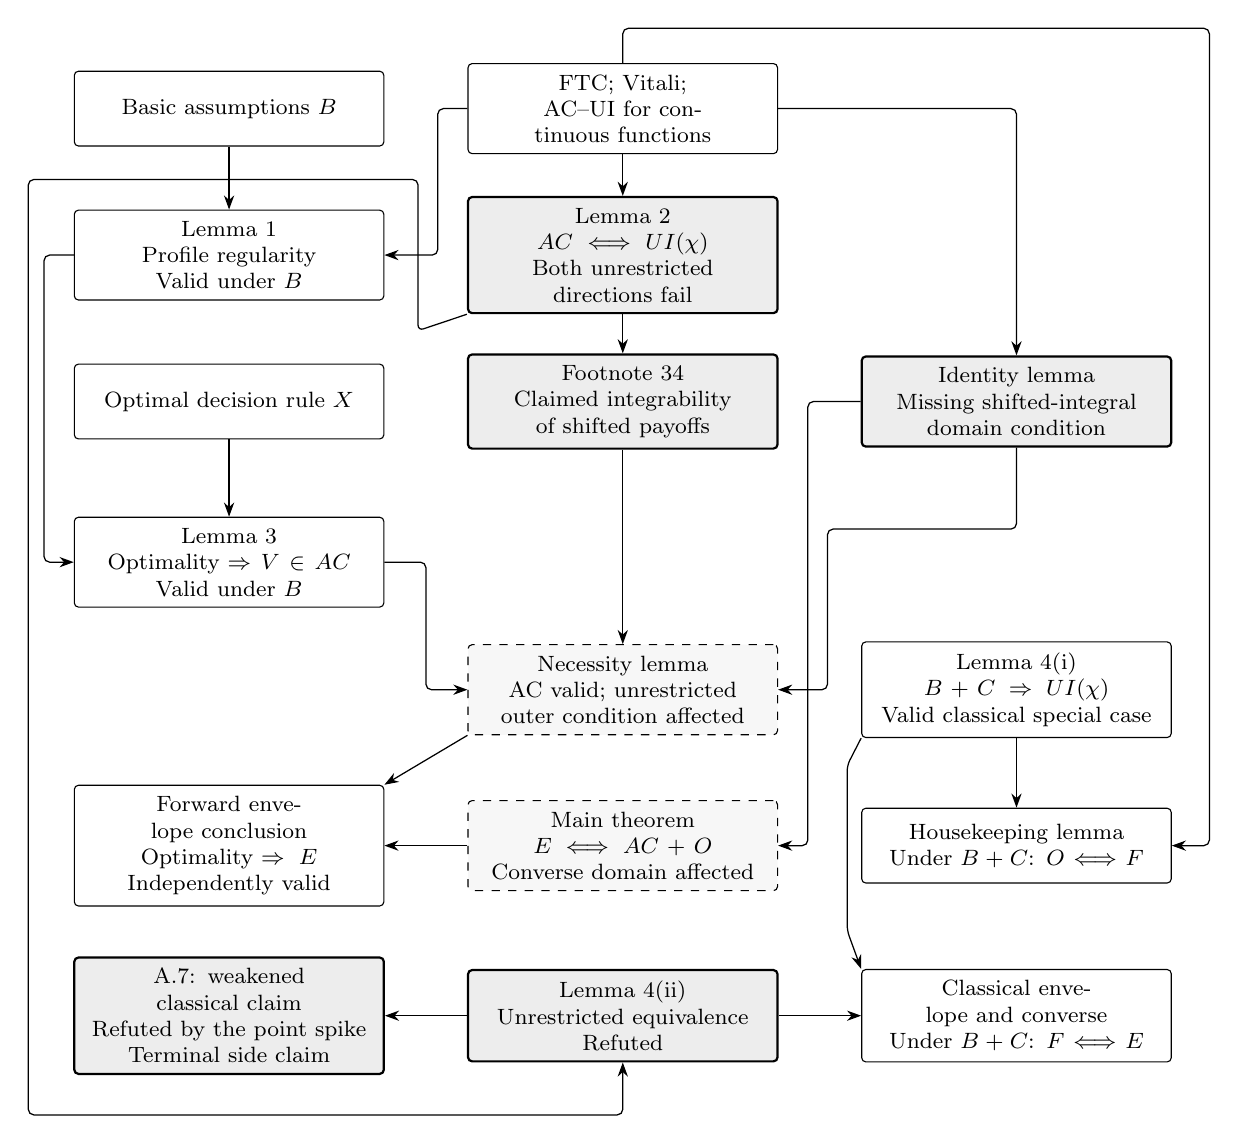
\begin{tikzpicture}[y=1.2cm]
\node[audit/node] (cB) at (-5,0) {Basic assumptions \(B\)};
\node[audit/node] (cBg) at (0,0) {FTC; Vitali;\\AC--UI for continuous functions};
\node[audit/node] (cL1) at (-5,-1.55) {Lemma 1\\Profile regularity\\Valid under \(B\)};
\node[audit/refuted] (cL2) at (0,-1.55) {Lemma 2\\\(AC\Longleftrightarrow UI(\chi)\)\\Both unrestricted directions fail};
\node[audit/node] (cOpt) at (-5,-3.1) {Optimal decision rule \(X\)};
\node[audit/refuted] (cFn) at (0,-3.1) {Footnote 34\\Claimed integrability\\of shifted payoffs};
\node[audit/refuted] (cId) at (5,-3.1) {Identity lemma\\Missing shifted-integral\\domain condition};
\node[audit/node] (cL3) at (-5,-4.8) {Lemma 3\\Optimality \(\Rightarrow V\in AC\)\\Valid under \(B\)};
\node[audit/qualified] (cNec) at (0,-6.15) {Necessity lemma\\AC valid; unrestricted\\outer condition affected};
\node[audit/node] (cL4a) at (5,-6.15) {Lemma 4(i)\\\(B+C\Rightarrow UI(\chi)\)\\Valid classical special case};
\node[audit/node] (cMS) at (-5,-7.8) {Forward envelope conclusion\\Optimality \(\Rightarrow E\)\\Independently valid};
\node[audit/qualified] (cMain) at (0,-7.8) {Main theorem\\\(E\Longleftrightarrow AC+O\)\\Converse domain affected};
\node[audit/node] (cHK) at (5,-7.8) {Housekeeping lemma\\Under \(B+C\): \(O\Longleftrightarrow F\)};
\node[audit/refuted] (cWeak) at (-5,-9.6) {A.7: weakened classical claim\\Refuted by the point spike\\Terminal side claim};
\node[audit/refuted] (cL4b) at (0,-9.6) {Lemma 4(ii)\\Unrestricted equivalence\\Refuted};
\node[audit/node] (cClass) at (5,-9.6) {Classical envelope and converse\\Under \(B+C\): \(F\Longleftrightarrow E\)};
\draw[audit/edge] (cB) -- (cL1);
\draw[audit/edge] (cBg.west) -- (-2.35,0) |- (cL1.east);
\draw[audit/edge] (cBg) -- (cL2);
\draw[audit/edge] (cBg.east) -| (cId.north);
\draw[audit/edge] (cBg.north) -- (0,0.85) -- (7.45,0.85) |- (cHK.east);
\draw[audit/edge] (cL1.west) -- (-7.35,-1.55) |- (cL3.west);
\draw[audit/edge] (cOpt) -- (cL3);
\draw[audit/edge] (cL2) -- (cFn);
\draw[audit/edge] (cL2.south west) -- (-2.6,-2.35) -- (-2.6,-0.75) -- (-7.55,-0.75) -- (-7.55,-10.65) -| (cL4b.south);
\draw[audit/edge] (cFn) -- (cNec);
\draw[audit/edge] (cL3.east) -- (-2.5,-4.8) |- (cNec.west);
\draw[audit/edge] (cId.south) -- (5,-4.45) -- (2.6,-4.45) |- (cNec.east);
\draw[audit/edge] (cId.west) -- (2.35,-3.1) |- (cMain.east);
\draw[audit/edge] (cNec.south west) -- (cMS.north east);
\draw[audit/edge] (cMain) -- (cMS);
\draw[audit/edge] (cL4a) -- (cHK);
\draw[audit/edge] (cL4a.south west) -- (2.85,-6.95) -- (2.85,-8.7) -- (cClass.north west);
\draw[audit/edge] (cL4b) -- (cClass);
\draw[audit/edge] (cL4b) -- (cWeak);
\end{tikzpicture}
\caption{Full core-theory dependencies, with published numbering.
\(B\) denotes the basic assumptions, \(C\) the classical assumptions, and
\(F\) the classical first-order condition. Arrows record cited proof inputs:
the unrestricted Lemma 4(ii) enters the published classical argument,
whose conclusion remains valid under \(B+C\). The A.7 weakening has no
outgoing arrow to either major theorem. Shaded boxes mark claims refuted
in their stated generality; dashed boxes mark conclusions requiring a
domain qualification or a different proof.}
\label{fig:audit-core}
\end{figure}
\FloatBarrier

\begingroup
\small
\setlength{\tabcolsep}{3pt}
\renewcommand{\arraystretch}{1.14}
\begin{longtable}{@{}>{\raggedright\arraybackslash}p{2.60cm}>{\raggedright\arraybackslash}p{6.30cm}>{\raggedright\arraybackslash}p{6.45cm}@{}}
\caption{Core theory: assumptions, conclusions, and assessed scope.}
\label{tab:dependency-core-full}\\
\toprule
Node & Assumptions and conclusion & Assessment \\
\midrule
\endfirsthead
\multicolumn{3}{@{}l}{\textit{Table \thetable\ continued}}\\
\toprule
Node & Assumptions and conclusion & Assessment \\
\midrule
\endhead
\midrule
\multicolumn{3}{r@{}}{\textit{Continued on next page}}\\
\endfoot
\bottomrule
\endlastfoot
FTC\par A.1
& $V\in\mathrm{AC}$ if and only if $V(t)=V(0)+\int_0^t g$ for some $g\in L^1$.
& \textbf{Standard theorem.} The representation holds at every type and need not survive an arbitrary almost-everywhere modification. \\
Vitali\par A.1
& A UI family of measurable, integrable functions converges almost everywhere: the limit is integrable and the integrals converge.
& \textbf{Standard theorem.} Measurability is required; domination alone does not imply it. \\
AC--UI\par A.1
& For a \emph{continuous} $V$, absolute continuity is equivalent to UI of its divided differences.
& \textbf{Standard theorem requiring continuity} of the specified pointwise representative. \\
Lemma 1\par A.2
& An absolutely equicontinuous family has absolutely continuous profiles and is uniformly equicontinuous.
& \textbf{Valid within $B$.} Differentiability supplies the profile continuity omitted from the standalone wording, which a singleton spike family refutes. \\
Lemma 3\par A.5
& Absolute equicontinuity and optimality of $X$ imply $V\in\mathrm{AC}$.
& \textbf{Valid within $B$.} Optimality gives continuity and the required value-difference bounds. Outside $B$, profile continuity is missing as in Lemma~1. \\
Lemma 2\par A.4, (i)$\Rightarrow$(ii)
& $B$ and $V\in\mathrm{AC}$ imply UI of $\{\chi_h\}$.
& \textbf{Counterexample.} The quadratic example has $V=0$ and nonmeasurable quotients at every relevant nonzero shift. \\
Lemma 2\par A.4, (ii)$\Rightarrow$(i)
& $B$ and UI of $\{\chi_h\}$ imply $V\in\mathrm{AC}$.
& \textbf{Counterexample.} The spike has integrable, UI quotients of zero $L^1$ norm but discontinuous $V$. \\
Footnote 34\par A.5
& Continuous $V$ and the forward direction of Lemma~2 imply integrability of the shifted payoffs.
& \textbf{Counterexample to integrability.} The paper derives integrability from the failed forward implication rather than assuming it. \\
Identity Lemma\par \S3.2; A.3
& $B$ and $V\in\mathrm{AC}$ imply that both sides of
$J'_{r,t}(0)=V(t)-V(r)-\int_r^t D$ are defined and equal.
& \textbf{Counterexample to well-definedness.} Shifted-integrand measurability is not ensured: the proof infers UI from integrable bounds without establishing measurability. \\
Necessity Lemma\par \S3.1; A.5
& $B$ and optimality of $X$ imply $V\in\mathrm{AC}$ and $O$.
& \textbf{Mixed scope.} AC is valid within $B$; the quadratic example defeats unconditional well-definedness of $O$. \\
Main theorem\par \S3.2, (i)$\Rightarrow$(ii)
& $B$, $V\in\mathrm{AC}$, and $O$ imply $E$.
& \textbf{Valid with the ordinary domain of $O$.} The proof must explicitly use the integrability supplied by $J$'s existence near zero, which $O$ already requires. \\
Main theorem\par \S3.2, (ii)$\Rightarrow$(i)
& $B$ and $E$ imply $V\in\mathrm{AC}$ and $O$.
& \textbf{Counterexample to unrestricted $E\Rightarrow O$.} $E$ implies AC but not shifted-integral existence. \\
Milgrom--Segal-type implication\par \S2.1
& $B$ and optimality of $X$ imply $E$.
& \textbf{Independently valid within $B$.} Lemma~3, optimality derivative bounds, and FTC suffice; the paper's route through $O$ has a domain gap. \\
Lemma 4(i)\par A.6
& $B+C$ imply UI of $\{\chi_h\}$.
& \textbf{Valid within $B+C$.} The classical assumptions supply measurability and a common bound. \\
Lemma 4(ii)\par A.6
& Under $B$, UI and almost-everywhere convergence of $\chi_h$ are equivalent to $V\in\mathrm{AC}$ and almost-everywhere existence of the imitation derivative.
& \textbf{Counterexamples in both directions.} The spike defeats (a)$\Rightarrow$(b); the quadratic example defeats (b)$\Rightarrow$(a), although its imitation derivative vanishes throughout the interior. \\
Housekeeping Lemma\par \S3.1
& $B+C$ imply $O\iff F$.
& \textbf{Valid within $B+C$.} Lemma~4(i) and Vitali justify interchanging differentiation and integration. \\
Classical envelope and converse\par \S2.2; A.7
& $B+C$ imply $F\iff E$.
& \textbf{Valid within $B+C$.} These assumptions exclude both counterexamples; the false unrestricted auxiliary equivalence does not refute this restricted conclusion. \\
Weakening claim\par A.7, final paragraph
& Replace $C$ by UI and almost-everywhere convergence of the deviation quotients, retaining $F\iff E$.
& \textbf{Counterexample.} The spike satisfies $F$ but not $E$, with all integrals defined. This extension is not upstream of the main or implementability theorem. \\
\end{longtable}
\endgroup
\FloatBarrier


\subsection{Mechanism design}
\label{sec:audit-mechanism-tables}

\paragraph{Notation.}
$A_0$ requires a partially ordered outcome set $\mathcal Y$, real payments,
and $f(y,\cdot,t)$ strictly decreasing and onto $\mathbb R$.
$R_Y$ is order density in itself, countable chain completeness, and chain
separability (Definition~5); the countable order-dense set may lie in the
ambient space.  $R_f$ is the payoff regularity in Definition~6: $f_3$ exists
and is bounded, its payment sections are continuous, and $f$ is jointly
continuous on each chain times payments and types.  Chains carry the
subspace topology inherited from the ambient strict-order-ray topology.
$SM$ and $SM^+$ denote the outer Spence--Mirrlees condition and its strict
version (Definition~7); ``increasing'' means weakly increasing. Their
quantification over arbitrary payment rules requires an integral-domain
qualification. IC means
$f(Y(t),P(t),t)\geq f(Y(r),P(r),t)$ for all reports $r$ and types $t$;
implementability means existence of such a payment rule.

The \emph{information primitives} below are a finite state space, a common
interior prior, and Borel distributions of posteriors with that mean.
Posterior value $v(\mu,t)$ has a bounded type derivative continuous in
$\mu$, and $f(y,p,t)=g(\int v(\mu,t)\,dy,p)$; $g$ is jointly continuous,
$g_1$ is bounded with continuous payment sections, and $g(v,\cdot)$ is
strictly decreasing and onto.  Under the literal definition, $SM^+$ has an
empty premise in a nonempty regular environment: constant allocation and
payment rules give an identically zero outer marginal gain, which is not
strictly single-crossing.

\begin{figure}[p]
\centering
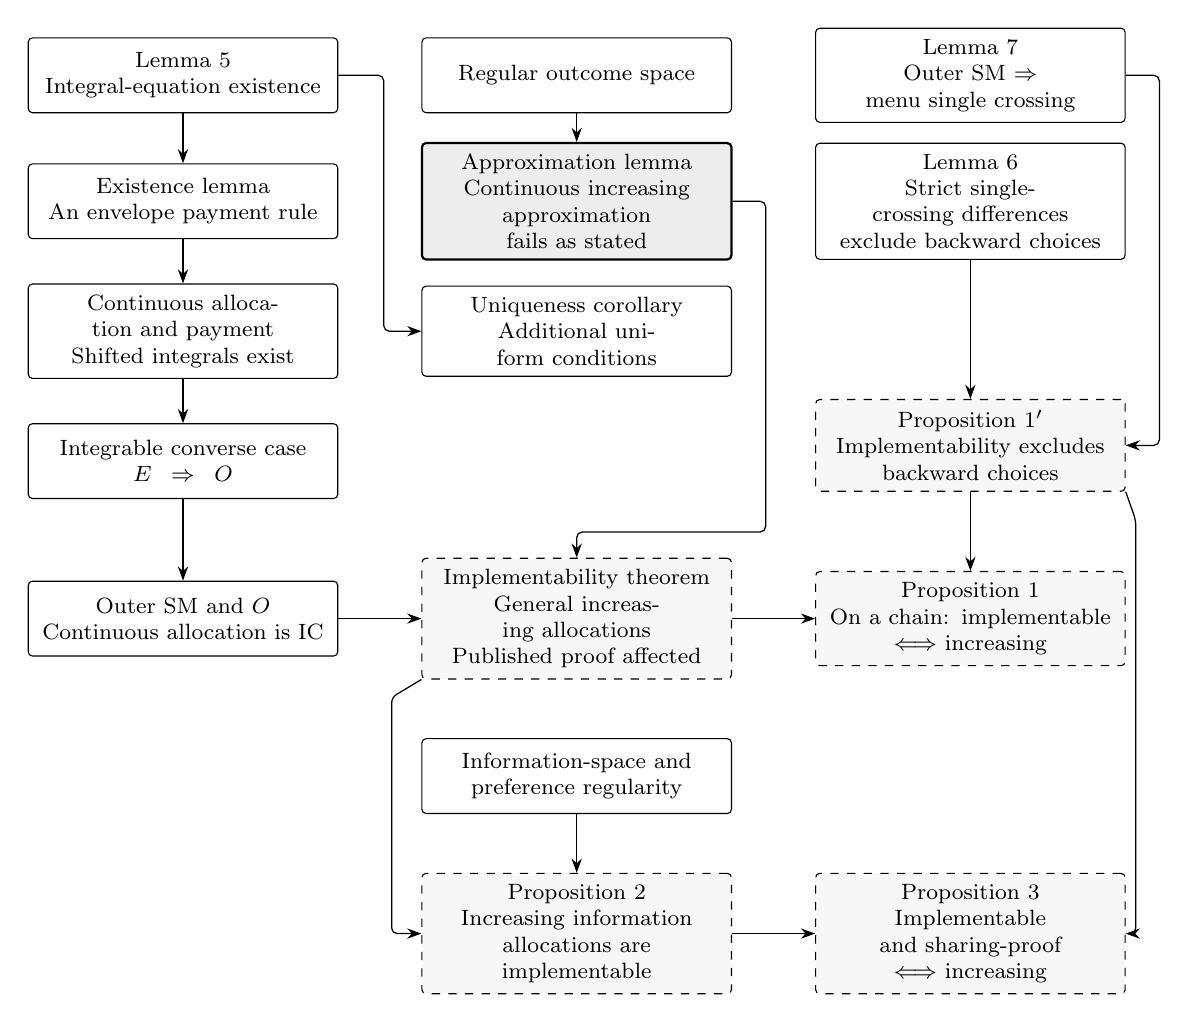
\begin{tikzpicture}
\node[audit/node] (aODE) at (-5,0) {Lemma 5\\Integral-equation existence};
\node[audit/node] (aRY) at (0,0) {Regular outcome space};
\node[audit/node] (aL7) at (5,0) {Lemma 7\\Outer SM \(\Rightarrow\)\\menu single crossing};
\node[audit/node] (aEx) at (-5,-1.6) {Existence lemma\\An envelope payment rule};
\node[audit/refuted] (aAp) at (0,-1.6) {Approximation lemma\\Continuous increasing\\approximation fails as stated};
\node[audit/node] (aL6) at (5,-1.6) {Lemma 6\\Strict single-crossing differences\\exclude backward choices};
\node[audit/node] (aCont) at (-5,-3.25) {Continuous allocation and payment\\Shifted integrals exist};
\node[audit/node] (aUn) at (0,-3.25) {Uniqueness corollary\\Additional uniform conditions};
\node[audit/node] (aCE) at (-5,-4.9) {Integrable converse case\\\(E\Rightarrow O\)};
\node[audit/qualified] (aP1p) at (5,-4.7) {Proposition \(1'\)\\Implementability excludes\\backward choices};
\node[audit/node] (aCIC) at (-5,-6.9) {Outer SM and \(O\)\\Continuous allocation is IC};
\node[audit/qualified] (aImp) at (0,-6.9) {Implementability theorem\\General increasing allocations\\Published proof affected};
\node[audit/qualified] (aP1) at (5,-6.9) {Proposition 1\\On a chain: implementable\\\(\Longleftrightarrow\) increasing};
\node[audit/node] (aInfo) at (0,-8.9) {Information-space and\\preference regularity};
\node[audit/qualified] (aP2) at (0,-10.9) {Proposition 2\\Increasing information\\allocations are implementable};
\node[audit/qualified] (aP3) at (5,-10.9) {Proposition 3\\Implementable and sharing-proof\\\(\Longleftrightarrow\) increasing};
\draw[audit/edge] (aODE) -- (aEx);
\draw[audit/edge] (aODE.east) -- (-2.45,0) |- (aUn.west);
\draw[audit/edge] (aEx) -- (aCont);
\draw[audit/edge] (aCont) -- (aCE);
\draw[audit/edge] (aCE) -- (aCIC);
\draw[audit/edge] (aRY) -- (aAp);
\draw[audit/edge] (aAp.east) -- (2.4,-1.6) -- (2.4,-5.8) -- (0,-5.8) -- (aImp.north);
\draw[audit/edge] (aCIC) -- (aImp);
\draw[audit/edge] (aL7.east) -- (7.4,0) |- (aP1p.east);
\draw[audit/edge] (aL6) -- (aP1p);
\draw[audit/edge] (aImp) -- (aP1);
\draw[audit/edge] (aP1p) -- (aP1);
\draw[audit/edge] (aInfo) -- (aP2);
\draw[audit/edge] (aImp.south west) -- (-2.35,-7.9) |- (aP2.west);
\draw[audit/edge] (aP2) -- (aP3);
\draw[audit/edge] (aP1p.south east) -- (7.1,-5.65) |- (aP3.east);
\end{tikzpicture}
\caption{Application dependencies. Arrows record the published proof route,
not refutations of final implementability conclusions. Continuous mechanisms
supply the repaired converse's integrability; the published passage to
general increasing allocations uses the false approximation lemma.
Separately, constant allocation and payment rules give zero marginal gain, violating the literal \emph{strict}
outer Spence--Mirrlees condition. This affects Lemma 7's strict version and
Propositions \(1',1,2,3\)'s premises, without refuting Lemma 6's usual strict
single-crossing argument. The uniqueness corollary is an optional side result.}
\label{fig:audit-application}
\end{figure}
\FloatBarrier

\begingroup
\small
\setlength{\tabcolsep}{3pt}
\renewcommand{\arraystretch}{1.14}
\begin{longtable}{@{}>{\raggedright\arraybackslash}p{2.60cm}>{\raggedright\arraybackslash}p{6.30cm}>{\raggedright\arraybackslash}p{6.45cm}@{}}
\caption{Mechanism design: assumptions, conclusions, and assessed scope.}
\label{tab:dependency-mechanism-full}\\
\toprule
Node & Assumptions and conclusion & Assessment \\
\midrule
\endfirsthead
\multicolumn{3}{@{}l}{\textit{Table \thetable\ continued}}\\
\toprule
Node & Assumptions and conclusion & Assessment \\
\midrule
\endhead
\midrule
\multicolumn{3}{r@{}}{\textit{Continued on next page}}\\
\endfoot
\bottomrule
\endlastfoot
Lemma 5\par B.1.1
& $\phi(\cdot,t)$ is continuous, strictly decreasing and onto; $\psi$ is bounded with continuous payment sections; both have Borel type sections. Then a $P$ solves
$\phi(P(t),t)=k+\int_0^t\psi(P(s),s)\,ds$.
& \textbf{Supported under the stated hypotheses} by a Carath\'eodory ODE argument with explicit measurability assumptions. \\
Existence Lemma\par B.1.1
& Payment sections are continuous, strictly decreasing and onto; $f_3$ is bounded with continuous payment sections. For the given $Y$, $f(Y(t),p,t)$ and $f_3(Y(t),p,t)$ are Borel in $t$ for every fixed $p$. Then an envelope payment exists for each initial value.
& \textbf{Supported under the stated hypotheses} by substitution in Lemma~5; measurability of the selected composites is explicit. \\
Uniqueness Corollary\par B.1.1
& The existence hypotheses hold; $f_3$ is uniformly Lipschitz in payment; utility decreases with payment at least at rate $M>0$. Then the envelope payment is unique.
& \textbf{Supported under the additional hypotheses} by ODE uniqueness; the implementability theorem does not require this node. \\
Approximation Lemma\par B.1.2
& $R_Y$ and increasing $Y$ yield an order-complete, order-dense, order-separable chain containing its image and continuous increasing $Y_n\to Y$ pointwise, preserving both endpoints.
& \textbf{Counterexample under the specified topology.} S.3, Step~4 identifies intrinsic chain and inherited ambient topologies; the $\mathbb R^2$ example refutes the resulting approximation. \\
Implementability Theorem\par \S4.3; B.1.3
& $A_0+R_Y+R_f+SM$ imply that every increasing allocation is implementable.
& \textbf{Proof gap for general allocations.} Continuous allocations have the required integral domain; the passage to arbitrary allocations uses the failed approximation lemma. No counterexample to the final conclusion is established here. \\
Lemma 6\par B.2
& On partially ordered actions and parameters, strict single-crossing differences imply that optimal selections cannot strictly reverse their order.
& \textbf{Supported under the stated hypotheses} by two optimality inequalities using ordinary strict single-crossing differences, independently of the defective literal $SM^+$ premise. \\
Lemma 7\par B.2
& $R_f+SM$, or its strict version, implies the corresponding single-crossing differences under any price menu.
& \textbf{Restricted construction is well-defined:} the proof's two-level step mechanisms have defined integrals. The strict version inherits $SM^+$'s empty premise. \\
Proposition $1'$\par B.2
& $A_0+R_f+SM^+$ imply that an implementable allocation cannot strictly reverse its order.
& \textbf{Empty strict premise as written.} Lemmas~6 and~7 give the argument independently of approximation. The defect concerns $SM^+$, not the usual strict single-crossing conclusion. \\
Proposition 1\par \S4.3; B.2
& $A_0+R_Y+R_f+SM^+$, with $\mathcal Y$ itself a chain, imply implementability if and only if the allocation is increasing.
& \textbf{Empty strict premise as written.} Sufficiency uses implementability; necessity uses Proposition~$1'$. The ambient $\mathbb R^2$ counterexample does not itself refute this chain case. \\
Proposition 2\par \S4.4
& The information primitives, space and payoff regularity, and $SM^+$ imply implementability of every Blackwell-increasing information allocation.
& \textbf{Empty strict premise; affected general proof.} The result uses the implementability theorem, whose proof gap does not establish a counterexample in this information-space case. \\
Proposition 3\par \S4.4; B.3
& In the same information environment, an allocation is implementable and sharing-proof if and only if it is increasing.
& \textbf{Empty strict premise; inherited proof issues.} Sufficiency uses Proposition~2; necessity uses Proposition~$1'$ and pairwise comparability of allocated outcomes. \\
\end{longtable}
\endgroup
\FloatBarrier


\subsection{Online supplement}
\label{sec:audit-supplement-tables}

DC means a difference of two continuous convex functions. A ``normalized
DC test'' has absolute value at most one, without separately bounding its
convex summands---a distinction essential to Lemma~S.2. Information-space
convergence uses the original statements' chain topology. ``Repair available''
means an independent argument for the indicated conclusion, not validation
of the published derivation.

\begin{figure}[p]
\centering
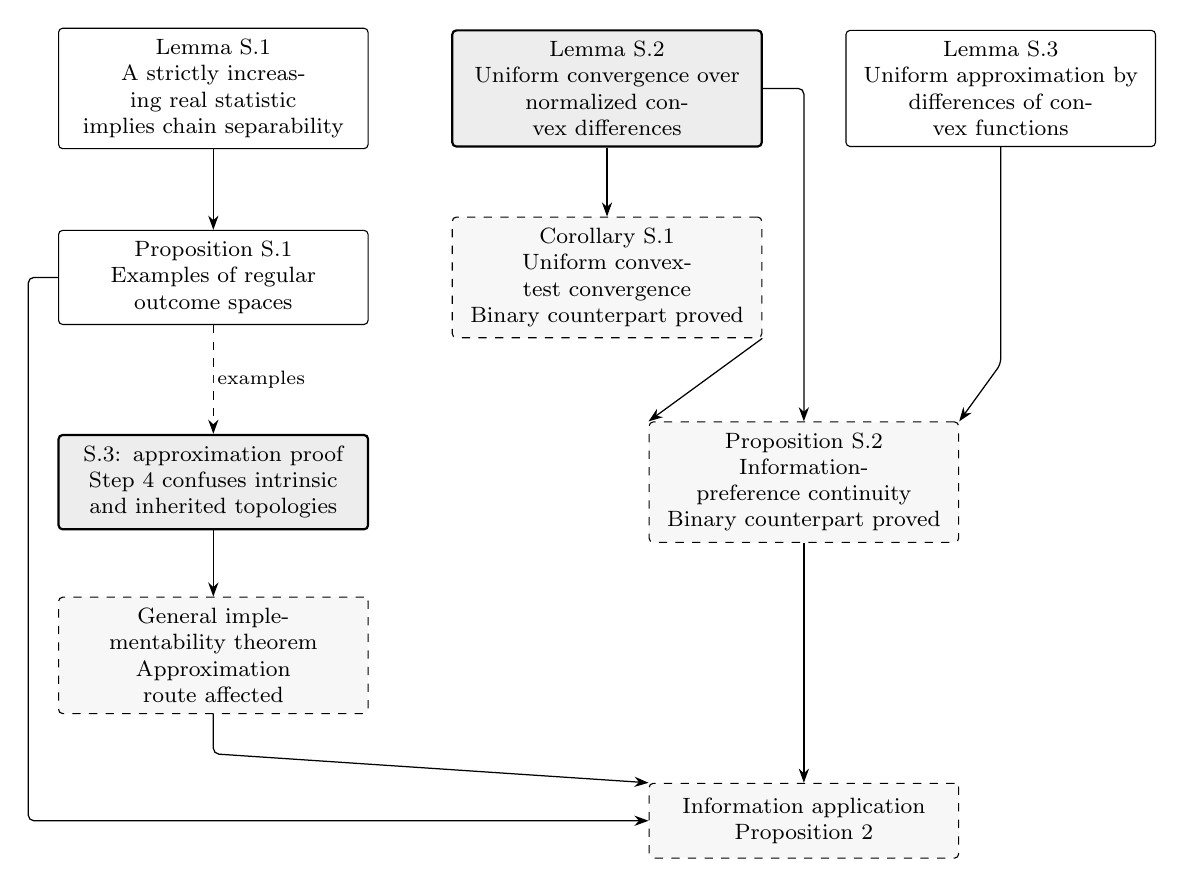
\begin{tikzpicture}
\node[audit/node] (sL1) at (-5,0) {Lemma S.1\\A strictly increasing real statistic\\implies chain separability};
\node[audit/refuted] (sL2) at (0,0) {Lemma S.2\\Uniform convergence over\\normalized convex differences};
\node[audit/node] (sL3) at (5,0) {Lemma S.3\\Uniform approximation by\\differences of convex functions};
\node[audit/node] (sP1) at (-5,-2.4) {Proposition S.1\\Examples of regular\\outcome spaces};
\node[audit/qualified] (sC1) at (0,-2.4) {Corollary S.1\\Uniform convex-test convergence\\Binary counterpart proved};
\node[audit/refuted] (sAp) at (-5,-5) {S.3: approximation proof\\Step 4 confuses intrinsic\\and inherited topologies};
\node[audit/qualified] (sP2) at (2.5,-5) {Proposition S.2\\Information-preference continuity\\Binary counterpart proved};
\node[audit/qualified] (sImp) at (-5,-7.2) {General implementability theorem\\Approximation route affected};
\node[audit/qualified] (sInfo) at (2.5,-9.3) {Information application\\Proposition 2};
\draw[audit/edge] (sL1) -- (sP1);
\draw[audit/edge,dashed] (sP1) -- node[audit/note,right] {examples} (sAp);
\draw[audit/edge] (sAp) -- (sImp);
\draw[audit/edge] (sL2) -- (sC1);
\draw[audit/edge] (sL2.east) -- (2.5,0) -- (sP2.north);
\draw[audit/edge] (sC1.south east) -- (sP2.north west);
\draw[audit/edge] (sL3.south) -- (5,-3.5) -- (sP2.north east);
\draw[audit/edge] (sP1.west) -- (-7.35,-2.4) |- (sInfo.west);
\draw[audit/edge] (sP2) -- (sInfo);
\draw[audit/edge] (sImp.south) -- (-5,-8.45) -- (sInfo.north west);
\end{tikzpicture}
\caption{Supplement dependencies, with published S-numbering. The dashed
``examples'' arrow marks Proposition S.1's examples satisfying the
approximation hypotheses; they are not prerequisites for the general proof.
Lemma S.2 has an explicit counterexample with supremum \(2\).
Independent binary-state proofs below repair Corollary S.1 and
Proposition S.2 for prior $1/2$ (with a common type-Lipschitz bound for
preference continuity), leaving S.3's approximation error unresolved.
The motivational, unnumbered quasilinear calculation in S.1 is omitted.
Figure~\ref{fig:audit-application} gives the additional qualification of
Proposition 2's strict outer Spence--Mirrlees premise.}
\label{fig:audit-supplement}
\end{figure}
\FloatBarrier

\begingroup
\small
\setlength{\tabcolsep}{3pt}
\renewcommand{\arraystretch}{1.14}
\begin{longtable}{@{}>{\raggedright\arraybackslash}p{2.60cm}>{\raggedright\arraybackslash}p{6.30cm}>{\raggedright\arraybackslash}p{6.45cm}@{}}
\caption{Online supplement: assumptions, conclusions, and assessed scope.}
\label{tab:dependency-supplement-full}\\
\toprule
Node & Assumptions and conclusion & Assessment \\
\midrule
\endfirsthead
\multicolumn{3}{@{}l}{\textit{Table \thetable\ continued}}\\
\toprule
Node & Assumptions and conclusion & Assessment \\
\midrule
\endhead
\midrule
\multicolumn{3}{r@{}}{\textit{Continued on next page}}\\
\endfoot
\bottomrule
\endlastfoot
Unnumbered calculation\par S.1
& Quasilinearity, an increasing allocation, envelope payments, and the stated single-crossing or monotone-type-derivative conditions imply IC.
& \textbf{Supported as the standard motivating argument;} it does not supply the general approximation step. \\
Lemma S.1
& A partially ordered set admitting a strictly increasing real-valued function is chain-separable.
& \textbf{Supported under the stated hypotheses:} each chain order-embeds in the real line. \\
Proposition S.1(a--c)
& $\mathbb R^n$, $\ell^1$, and $L^1$, with their coordinate or almost-everywhere orders, satisfy $R_Y$.
& \textbf{Supported under the usual nonempty-chain convention} by midpoints, countable order bounds, and strictly increasing integral or coordinate functionals. \\
Proposition S.1(d)
& Finite-state posterior distributions with a fixed mean, ordered by Blackwell informativeness, satisfy $R_Y$.
& \textbf{Supported under the stated hypotheses} by mixtures, weak compactness, convex order, and strict Jensen inequalities. \\
Proposition S.1(e)
& The open subintervals of $(0,1)$, together with the empty set and ordered by inclusion, satisfy $R_Y$.
& \textbf{Supported under the stated conventions} by interval unions, interiors of intersections where required, and length. \\
Approximation proof\par S.3
& A regular outcome space and an increasing allocation admit continuous increasing approximations preserving endpoints.
& \textbf{Counterexample.} Step~4 identifies intrinsic chain and inherited ambient topologies; the $\mathbb R^2$ example refutes the stated approximation. \\
Lemma S.2\par S.4
& Convergence $y_n\to y$ on a chain of posterior distributions implies uniform convergence of their integrals over all normalized continuous DC tests.
& \textbf{Explicit counterexample.} For two-point mean-preserving spreads converging to $\delta_{1/2}$, a triangular test gives supremum integral discrepancy $2$ for every $n$, with all expressions defined. \\
Corollary S.1\par S.4
& Under the same convergence assumptions, integrals converge uniformly over continuous convex tests taking values in $[-1,1]$.
& \textbf{Proof gap; repair available.} The derivation uses Lemma~S.2; an independent order-sandwich argument below proves this narrower conclusion for binary states with prior $1/2$. \\
Lemma S.3\par S.4
& Every continuous function on the simplex can be uniformly approximated by continuous DC functions.
& \textbf{Supported under the stated hypotheses} by the DC algebra and Stone--Weierstrass. \\
Proposition S.2\par S.4
& The information primitives imply joint continuity of payoff on each chain times payments and types.
& \textbf{Proof gap; repair available.} The published proof uses Lemma~S.2. Fixed-test continuity and a common type-Lipschitz bound give the binary-state repair below for prior $1/2$. \\
\end{longtable}
\endgroup
\FloatBarrier


\clearpage
\section{Additional counterexamples and proof details}\label{app:audit-witnesses}
Theorem~\ref{thm:counter} and Proposition~\ref{prop:compactexample}
establish the quadratic measurability counterexample.  This appendix
gives the other witnesses in Table~\ref{tab:audit-impact}, each with a
complete Lean certificate including its hypotheses.


% Additional counterexamples with complete Lean certificates.

\subsection{A point modification in Lemma 2}
\label{app:audit-spike}

\paragraph{Claim and counterexample.}
Lemma 2 of \citet[Appendix A.4]{Sinander2022} asserts that, under the
basic assumptions, absolute continuity of the selected value is
equivalent to uniform integrability of the selected imitation
quotients.  Take $\mathcal X=\{0,1\}$, $t_0=1/2$, and
\[
 f(x,t)=x,\qquad X(t)=\ind_{\{t_0\}}(t),\qquad
 V(t)=f(X(t),t)=\ind_{\{t_0\}}(t).
\]
Every fixed-action type profile is constant, so its type derivative and
divided differences vanish, verifying the basic assumptions.
For every $h\ne0$, wherever both arguments lie in $[0,1]$,
\[
 \chi_h(s)=\frac{f(X(s+h),s)-f(X(s),s)}h
 =\frac{\ind_{\{t_0-h\}}(s)-\ind_{\{t_0\}}(s)}h.
\]
This measurable function is supported on at most two points.
Extending it by zero outside its domain gives $\int |\chi_h|=0$ for
every $h$, hence uniform integrability.  Yet $V$ is discontinuous at
$t_0$ and therefore not absolutely continuous.  This refutes Lemma 2's
uniform-integrability-to-absolute-continuity implication: its proof
invokes the AC--UI lemma of Appendix A.1 without establishing the
required continuity of the selected value.

\paragraph{Scope.}
Every shifted payoff integral exists and is zero, so the outer
first-order condition holds.  The envelope identity fails at $t_0$:
its sides, normalized at zero, are $1$ and $0$.
For each $s\ne t_0$, the selected payoff is constant under sufficiently
small shifts, so the imitation derivative is zero.  Thus the quotients
converge almost everywhere and the classical first-order condition
holds.  This also refutes Lemma~4(ii)(a)$\Rightarrow$(b) and the final
paragraph of the original Appendix~A.7, which proposes uniform
integrability and almost-everywhere quotient convergence as sufficient
replacements for the classical assumptions.
This does not refute the main equivalence: its outer-condition side
requires absolute continuity of $V$, which fails here.
The Lean module \texttt{SpikeCounterexample} represents the actions by
\texttt{Bool}; \texttt{complete\_counterexample} certifies the actual
quotient suprema, uniform integrability, imitation derivative, outer
condition, failure of absolute continuity, and failed envelope equality.

\subsection{The ambient order topology in the approximation lemma}
\label{app:audit-order-topology}

\paragraph{The two topologies.}
The approximation lemma in \citet[Appendix B.1.2]{Sinander2022} gives
its chain $C$ the relative topology inherited from the ambient partially
ordered outcome space.  Definition 6, footnote 14, defines the ambient
order topology by strict order rays.  The inherited topology need not
equal the chain's own order topology.

\paragraph{Counterexample.}
Let $\mathcal Y=\R^2$ have the coordinatewise order: $x\prec y$ means
$x_i\le y_i$ in both coordinates and $x\ne y$.
This outcome space is regular, as Proposition S.1(a) also records:
midpoints give order density, coordinatewise suprema and infima give
the requisite chain completeness, and the strictly increasing map
$(y_1,y_2)\mapsto y_1+y_2$ gives chain separability.
For any $a=(a_1,a_2)$, four open strict order rays intersect in $\{a\}$:
\[
\begin{split}
 &\{x:(a_1-1,a_2)\prec x\}
 \cap\{x:(a_1,a_2-1)\prec x\}\\
 &\hspace{8mm}\cap\{x:x\prec(a_1+1,a_2)\}
 \cap\{x:x\prec(a_1,a_2+1)\}=\{a\}.
\end{split}
\]
The first two require $x_i\ge a_i$ and the last two $x_i\le a_i$;
$a$ belongs to all four.  Thus the ambient topology and every inherited
chain topology are discrete.

For the increasing allocation $Y(t)=(t,0)$, the lemma requires
continuous maps $Y_n:[0,1]\to C$ with $Y_n(0)=(0,0)$ and
$Y_n(1)=(1,0)$.  A continuous image of a connected interval in a
discrete space is a singleton, so no such maps exist, even without
pointwise convergence.  Step 4 of Supplement S.3 identifies the chain
with an interval in its own order topology; this does not establish
the claimed homeomorphism in the inherited topology.

\paragraph{Scope and repair.}
This refutes the approximation lemma and invalidates its use in Step 2
of the implementability proof; it does not exhibit a nonimplementable
increasing allocation satisfying the other assumptions.
A repair using intrinsic chain order topologies must also impose
preference continuity in those topologies; continuity in a finer,
possibly discrete, inherited topology is insufficient.
The module \texttt{OrderTopologyAudit} certifies regularity of
$\mathbb R^2$, the generated and inherited topologies, and the obstruction
for every containing chain in
\texttt{complete\_\allowbreak approximation\_\allowbreak counterexample}.

\subsection{Constant mechanisms and the strict outer condition}
\label{app:audit-strict-sm}

\paragraph{Literal obstruction.}
Definition 7 of \citet[Section 4.2]{Sinander2022} quantifies over every
increasing allocation $Y$ and payment schedule $P$.  Its strict version
requires the outer derivative to be strictly single-crossing in type
displacement: footnote 17 requires
$q(n)\ge0\Rightarrow q(n')>0$ for $n<n'$.
On any nonempty outcome space, fix $y_0,p_0$ and take the increasing
allocation $Y(s)=y_0$ with $P(s)=p_0$.  For $r=1/4$, $t=3/4$ and
sufficiently small displacements,
\[
 \int_r^t f(Y(s+m),P(s+m),s+n)\,ds
 =\int_r^t f(y_0,p_0,s+n)\,ds,
\]
independently of $m$.  The integral exists by continuity of the
fixed-outcome, fixed-payment type profile on a compact interval.
Its upper $m$-derivative is zero for every $n$ in a nondegenerate
neighborhood of zero.  Two distinct such displacements contradict
strict single-crossing.

\paragraph{Scope.}
The literal strict condition with nonempty outcomes and continuous fixed profiles yields an empty domain with the given universal quantifiers and weak meaning of increasing; this is a fault in the definition, but it does not refute any conditional theorem, nonstrict condition, or classical strict single crossing preferences.  The test for the strict condition requires qualification or reformulation.  The witness is constant, so measurable payments don't help.  \texttt{StrictOuterSM} proves the witness integrable on the tested window, calculates the upper derivative by a limsup, and proves \texttt{ordinary\_strict\_condition\_impossible} even when the test is restricted to paths with integrable payoffs and ordinary finite derivatives.  \texttt{literal\_strict\_condition\_impossible} stores the totalized encoding separately; the obstruction requires no identification with undefined expressions on other paths.

\subsection{An explicit counterexample to Supplement Lemma S.2}
\label{app:audit-dc-tests}

\paragraph{Statement under audit.}
Supplement Lemma S.2 of \citet{Sinander2022} (Lemma 9 in Appendix N of
the June 2022 preprint) asserts that convergence along a Blackwell
chain in the inherited ambient order topology implies convergence in
\[
 d(y,z)=\sup_{\substack{v^+,v^-\text{ continuous convex}\\
                        |v^+-v^-|\le1}}
 \left|\int (v^+-v^-)\,d(y-z)\right|.
\]
The following chain converges in that topology but has distance $2$
at every term.

\paragraph{A convergent Blackwell chain.}
Identify the binary posterior simplex with $[0,1]$.  At prior $p=1/2$,
let $\varepsilon_n=1/(4(n+1))$ for $n=0,1,\ldots$; these radii lie in
$(0,1/2)$ and decrease to zero.  Define the Bayes-plausible laws
\[
 y=\delta_p,\qquad
 y_n=\tfrac12\delta_{p-\varepsilon_n}
       +\tfrac12\delta_{p+\varepsilon_n}.
\]
By Jensen's inequality, $y$ is least informative among laws with this
mean.  Convexity at the two symmetric support points shows that $y_n$
decreases in Blackwell order, so these laws form a chain.

To prove ambient convergence, fix any $z$ strictly above $y$.
Since $z$ is not concentrated at its mean, it has a measurable partition
of probabilities $w,1-w\in(0,1)$ with distinct conditional means
$a<b$ satisfying $wa+(1-w)b=p$.  Jensen's inequality on each part gives
\[
 wv(a)+(1-w)v(b)\le\int v\,dz
\]
for every continuous convex $v$.  For
$0\le\varepsilon\le\min\{w(b-a),(1-w)(b-a)\}$, put
$d=\varepsilon/(b-a)$.  The points $p-\varepsilon,p+\varepsilon$ are
convex combinations of $a,b$ with respective weights $w+d,w-d$ on $a$.
Averaging the convexity inequalities gives
\[
 \tfrac12v(p-\varepsilon)+\tfrac12v(p+\varepsilon)
 \le wv(a)+(1-w)v(b)\le\int v\,dz.
\]
Hence $y_n\preceq z$ eventually.  Since $z\not\preceq y$, some
continuous convex $v$ satisfies $\int v\,dy<\int v\,dz$.
Continuity gives $\int v\,dy_n\to\int v\,dy$, so
$z\not\preceq y_n$ eventually.  Thus $y_n\prec z$ eventually.
Every subbasic neighborhood of the minimum $y$ is a lower ray
$\{w:w\prec z\}$ with $y\prec z$; no upper ray contains $y$.
The sequence is eventually in each such ray and each finite intersection,
proving convergence in the ambient order topology and its restriction
to the displayed chain.

\paragraph{A distance that remains exactly two.}
Define the continuous piecewise-linear test
\[
 w_n(x)=
 \frac{|x-(p-\varepsilon_n)|+|x-(p+\varepsilon_n)|}
      {\varepsilon_n}
 -\left(\frac{2|x-p|}{\varepsilon_n}+1\right).
\]
Both terms are continuous convex functions.  Their difference satisfies
$|w_n|\le1$, equals $1$ at $p$, and equals $-1$ at $p\pm\varepsilon_n$.
Hence
\[
 \int w_n\,dy_n=-1,\qquad \int w_n\,dy=1.
\]
Thus $d(y_n,y)\ge2$.  Expectations of any function bounded in absolute
value by one differ by at most two, so $d(y_n,y)=2$ for every $n$.
All integrals are finite probability integrals.
Lemma S.2's proof wrongly infers that an order interval lies in a
$d$-ball because its endpoint does: $d$ is not monotone along Blackwell
intervals.  The modules \texttt{InformationWitness} and
\texttt{InformationCounterexample} prove these claims for actual
probability measures.  Their
\texttt{complete\_\allowbreak information\_\allowbreak counterexample} certifies the full ambient
strict-ray topology, the inherited chain topology, convex test
decompositions, integrability, and exact supremum; Jensen domination
and convergence are proved, not assumed.

\paragraph{Binary continuity repair.}
The false uniform DC-distance claim does not itself refute preference
regularity for selling information.  In the binary setting with prior
$1/2$, independent machine-checked continuity repairs hold.
Let $V(\mu,t)$ be continuous and convex in $\mu$ for each $t\in[0,1]$
and uniformly $L$-Lipschitz in type.  Put
$H(y,t)=\int V(\mu,t)\,dy(\mu)$.  Then
\[
 |H(y',t')-H(y,t)|
 \le L|t'-t|
   +\left|\int V(\mu,t)\,d(y'-y)(\mu)\right|.
\]
Each fixed continuous convex test has continuous expectation in the
ambient strict-ray topology.  Indeed, mix $y$ with weight $0<\alpha<1$
of the least or most informative law.  Unless $y$ is already the
respective extremum, these mixtures lie strictly below or above $y$;
the resulting open rays sandwich nearby expectations.  At an extremum,
the corresponding bound holds globally.  For continuous convex tests valued in
$[-1,1]$, the difference bound is $2\alpha$, uniformly over the class.
Thus this topology gives uniform convergence over normalized continuous
convex tests, though not over normalized differences of convex functions.

Fixed-test continuity and the common type-Lipschitz bound give joint
continuity of $H$ and of every continuous monetary aggregation
$g(H(y,t),p)$, also on every chain with the inherited topology.
The modules \texttt{InformationMixtures} and
\texttt{InformationContinuity} prove these binary repairs using actual
mixtures of probability laws in
\texttt{convexDiscrepancy\_tendsto},
\texttt{convex\_expectation\_continuous}, and
\texttt{information\_utility\_jointly\_continuous}.
These results neither formalize the supplement's general finite-state
conclusions nor repair the separate approximation-topology issue.




\clearpage
\section{Machine-checked supplement}\label{app:formal}
The accompanying 16-module Lean~4 project proves declarations representing all nine numbered mathematical results (four in the main text and five in Appendix~\ref{app:representation}) and the four counterexamples in Appendix~\ref{app:audit-witnesses}. Its 241 public theorem declarations, including supporting results, were checked with Lean~4.30.0 and mathlib revision \texttt{c5ea00351c28e24afc9f0f84379aa41082b1188f}. The build and axiom audit pass without proof placeholders or added axioms; foundational dependencies are propositional extensionality, classical choice, and quotient soundness. The source-paper dependency maps are a bibliographic and logical audit, not a formalization of every cited result.

The declaration \texttt{complete\_counterexample} supplies a single witness satisfying differentiability, uniform Lipschitz continuity, optimality, the envelope formula, quotient-supremum uniform integrability, and deviation nonintegrability. The non-Lebesgue-measurable set comes from a rational-equivalence transversal. The declaration \texttt{repaired\_converse} combines measurable-profile representation, the shifted-integral identity, unit-interval domain reduction, endpoint extension, and absolute continuity, deriving derivative measurability and integrability.

The formal integral has a default value outside its integrability domain. The measurability counterexample proves failure of almost-everywhere measurability and integrability; the repaired identity establishes interval integrability. For an interval profile $p$, the interior derivative is that of $v\mapsto p(c(v))$, where $c(v)=\min\{1,\max\{0,v\}\}$. This is the usual interior derivative because $c$ locally equals the identity; endpoint differentiability is not required. For type-domain reduction, profiles and selected types extend to the real line by clamping into $[0,1]$. For each interior integration interval, the extension agrees with the economic payoff throughout that interval for all shifts near zero. A separate claim map records each numbered result's hypotheses and declarations. Bibliographic interpretation and economic discussion remain outside the formal scope.

\clearpage
\begin{thebibliography}{9}
\bibitem[Milgrom and Segal(2002)]{MilgromSegal2002}
Milgrom, P., and I. Segal (2002): ``Envelope Theorems for Arbitrary Choice Sets,'' \textit{Econometrica}, 70(2), 583--601. \href{https://doi.org/10.1111/1468-0262.00296}{doi:10.1111/1468-0262.00296}.
\bibitem[Sinander(2022)]{Sinander2022}
Sinander, L. (2022): ``The Converse Envelope Theorem,'' \textit{Econometrica}, 90(6), 2795--2819. \href{https://doi.org/10.3982/ECTA18119}{doi:10.3982/ECTA18119}.
\bibitem[Sinander(2022, Supplement)]{Sinander2022supp}
Sinander, L. (2022): Supplement to ``The Converse Envelope Theorem,'' \textit{Econometrica}, Online Supplemental Material, Sections S.1--S.4. \href{https://www.econometricsociety.org/publications/econometrica/2022/11/01/The-Converse-Envelope-Theorem/supp/ecta200504-sup-0001-onlineappendix.pdf}{Online supplement}.
\end{thebibliography}
\end{document}
